%%%%%%%%%%%%%%%%%%%%%%%%%%%%%%%%%%%%%%%%%%%%%%%%%%%%%%%%%%%%%%%
%%%%%%%%%%%%%%%%%%%%%%%%%%%%%%%%%%%%%%%%%%%%%%%%%%%%%%%%%%%%%%%
% Appendices
%%%%%%%%%%%%%%%%%%%%%%%%%%%%%%%%%%%%%%%%%%%%%%%%%%%%%%%%%%%%%%%
\par\noindent\textbf{\huge{\color{blue}Appendices}}
\addcontentsline{toc}{chapter}{Appendices} % Adds to Table of Contents
\markboth{Appendices}{} % Updates headers with "Appendices" 

\vspace{3cm}

% Add your appendices content here
Your appendices content goes here...

\begin{figure}[H]
    \centering
    \includegraphics[width=17cm,height=7cm]{MainLayout/Images/chapter8/kernels_segments_subjects_controls.jpg}
    \caption{Main Title for First Image \\ \small Subtitle for the first graphic.}
    \label{fig:kernels_segments_subjects_controls}
\end{figure}

\begin{figure}[H]
    \centering
    \includegraphics[width=17cm,height=7cm]{MainLayout/Images/chapter8/kernels_segments_subjects_patients.jpg}
    \caption{Main Title for First Image \\ \small Subtitle for the first graphic.}
    \label{fig:kernels_segments_subjects_patients}
\end{figure}

\begin{figure}[H]
    \centering
    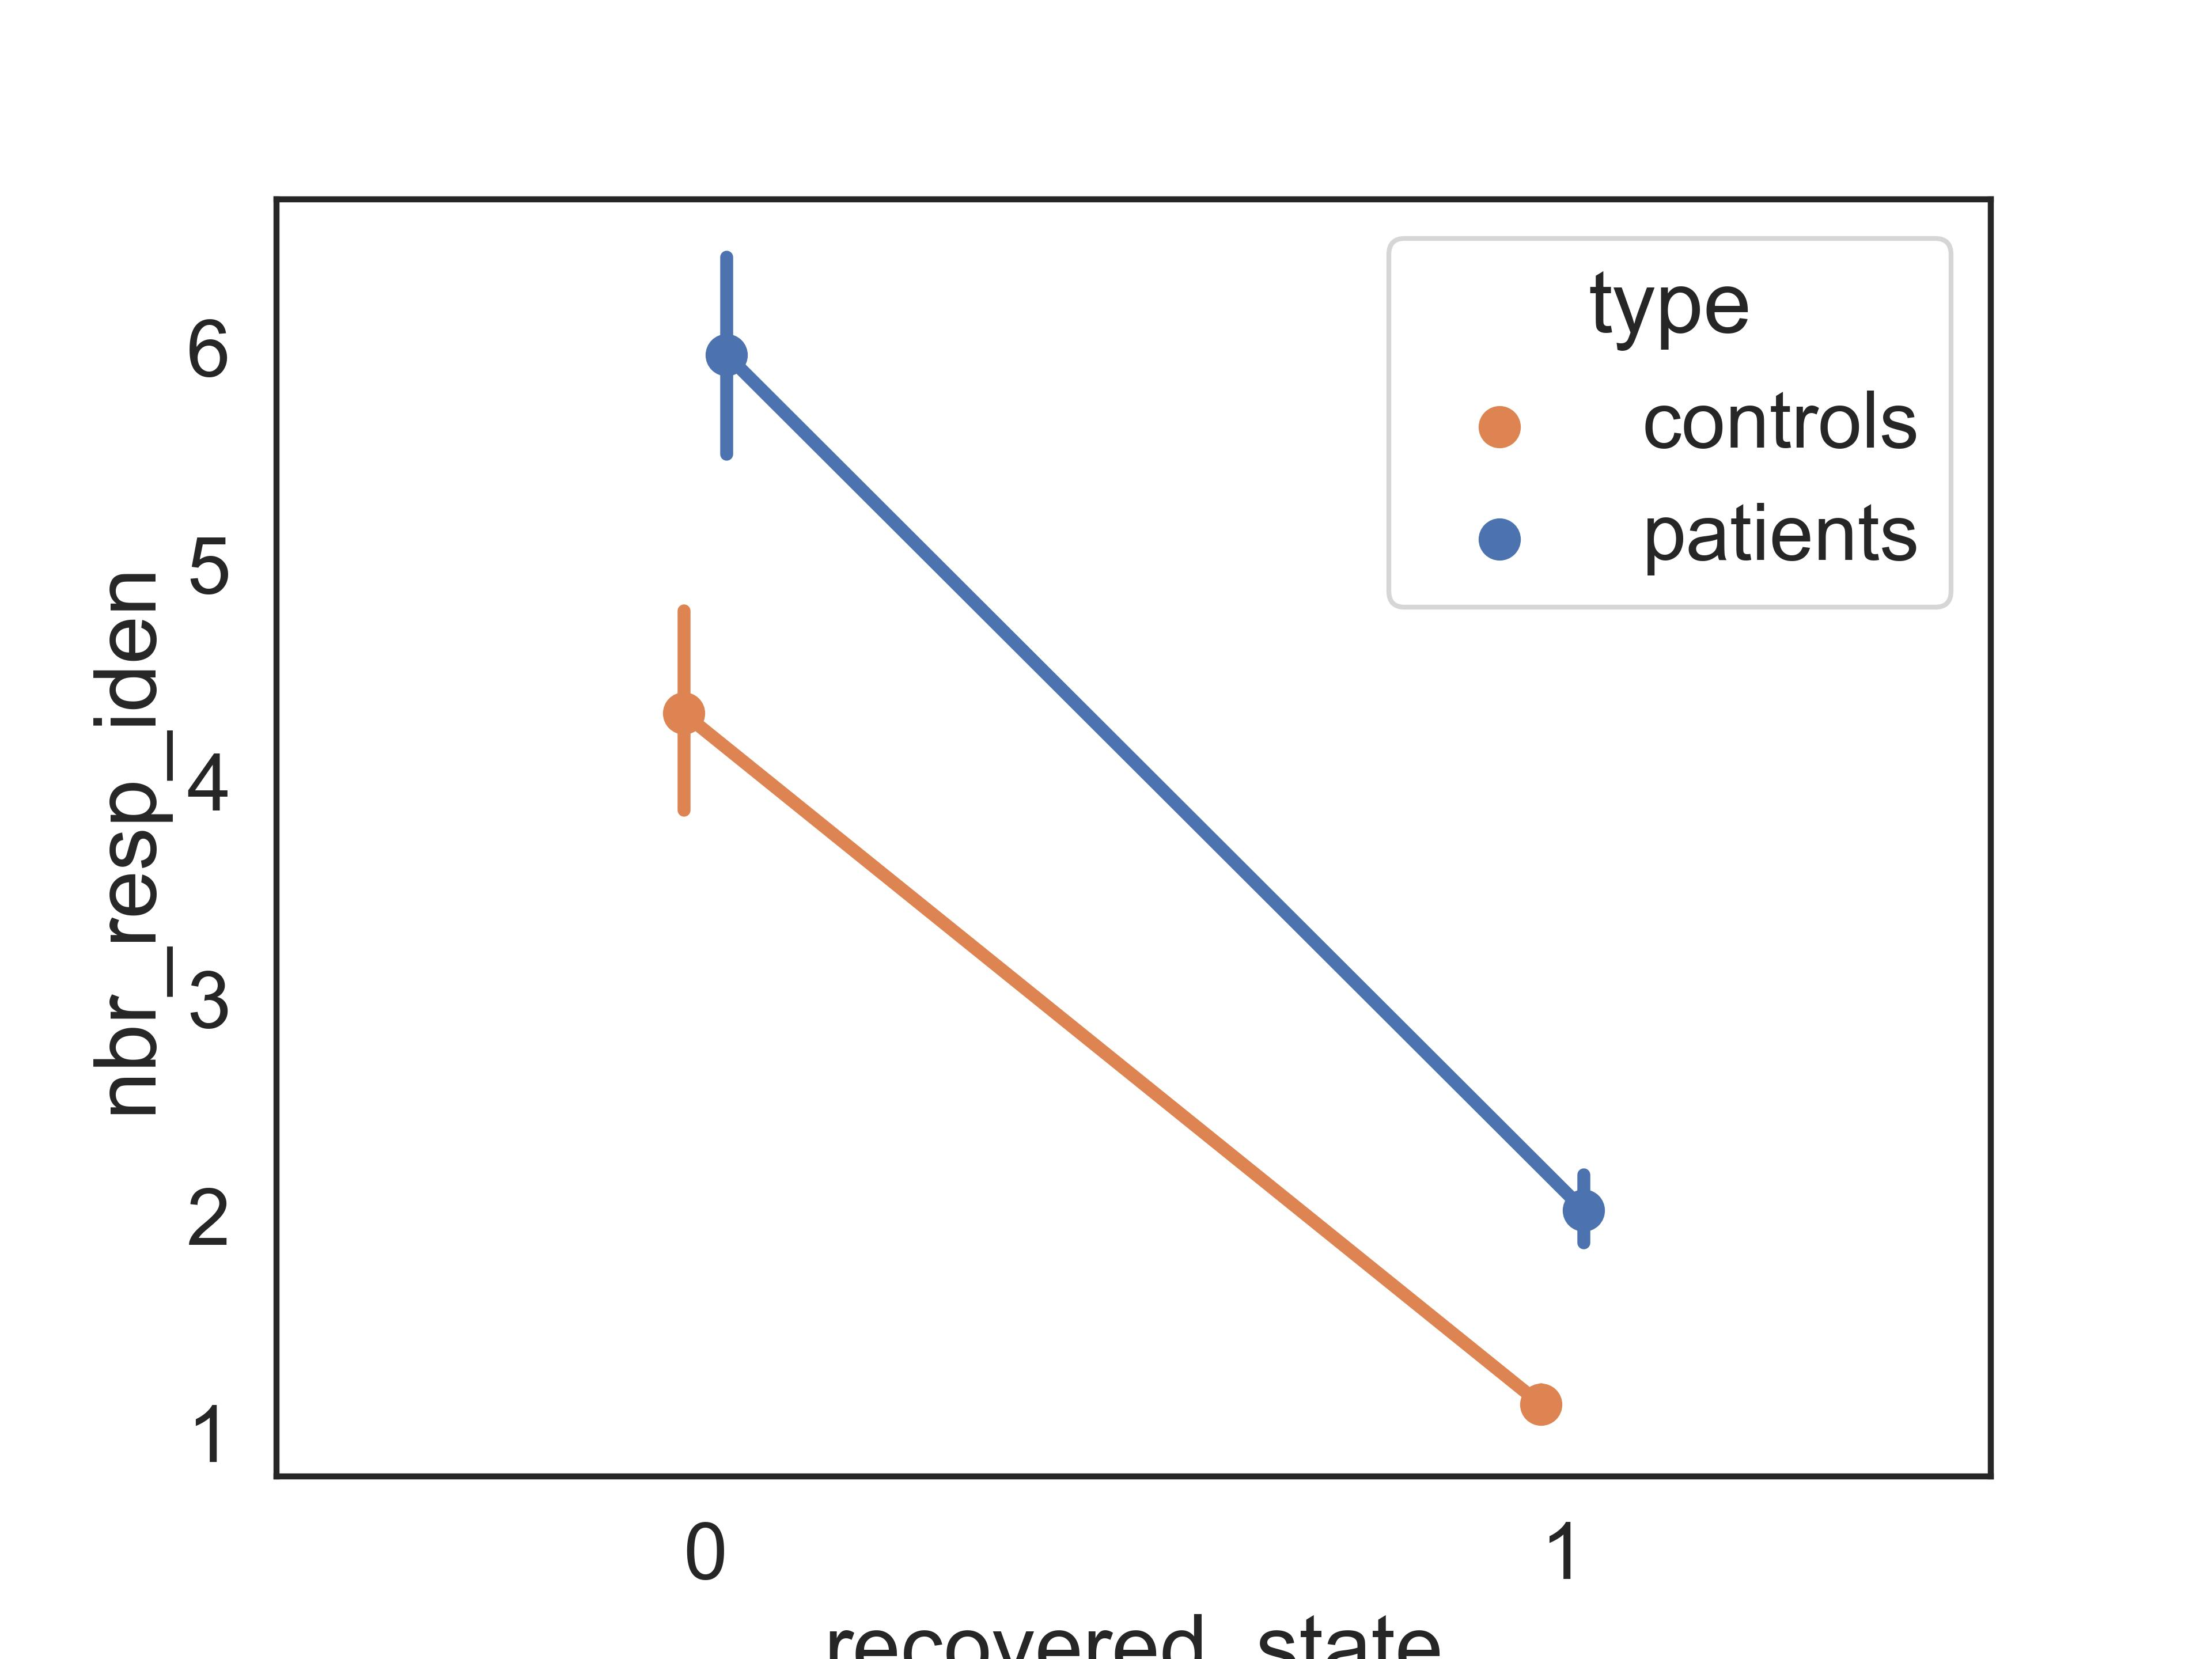
\includegraphics[width=12cm,height=7cm]{MainLayout/Images/chapter9/nbr_resp_iden.jpg}
    \caption{Main Title for First Image \\ \small Subtitle for the first graphic.}
    \label{fig:nbr_resp_iden}
\end{figure}
\vspace{1cm}

% Optional: Add a blank page if printing double-sided
\newpage
\thispagestyle{empty} % Ensures the blank page has no header/footer
\hspace{1cm} % Leaves the blank page empty

\newpage